%!TEX encoding = UTF-8 Unicode
%!TEX root = ../lect-week07.tex

%%%


%\begin{Slide}{TODO: Begrepp att förklara}
%  Tänk igenom ordningen:
%  \begin{itemize}
%    \item OO, arv, supertyp, subtyp, bastyp, polymorfism, ... 
%  \end{itemize}
%\end{Slide}

\ifkompendium\else

\Subsection{Arv och nyckelordet \texttt{extends}}

\begin{Slide}{Vad är arv?}

\begin{minipage}{0.4\textwidth}
\raggedright Med arv kan man beskriva relationen \\
$X$ \Emph{är en} $Y$

\end{minipage}
\begin{minipage}{0.4\textwidth}
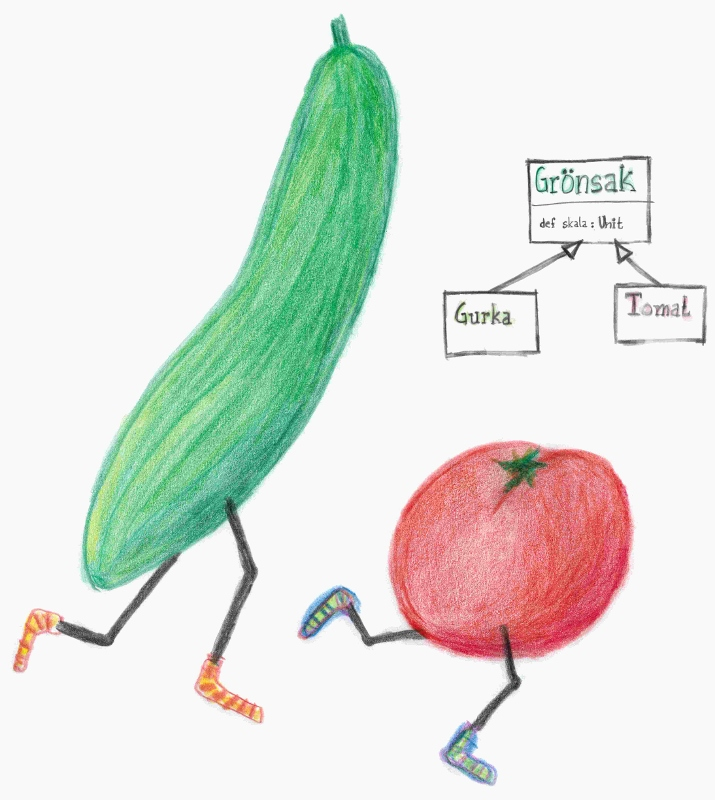
\includegraphics[width=1.5\textwidth]{../img/gurka-tomat-715x800}
\end{minipage} 
\end{Slide}


\begin{Slide}{Varför behövs arv?}
\begin{itemize}
\item Man kan använda arv för att dela upp kod i: 
\begin{itemize}
\item \Emph{generella} (gemensamma) delar och 
\item \Emph{specifika} (specialanpassade) delar.
\end{itemize}

\item Man kan åstadkomma \Emph{kontrollerad flexibilitet}: 
\begin{itemize}
\item Klientkod kan \Emph{utvidga} \Eng{extend} ett givet API med egna specifika tillägg.
\end{itemize}

\item Man kan använda arv för att deklarera en gemensam \Emph{bastyp} så att generiska samlingar kan ges en mer specifik elementtyp. 
\begin{itemize}
\item Det räcker att man vet bastypen för att kunna anropa gemensamma metoder på alla element i samlingen.
\end{itemize}
\end{itemize}
\end{Slide}


\begin{Slide}{Behovet av gemensam bastyp}
\begin{REPL}
scala> class Gurka(val vikt: Int)

scala> class Tomat(val vikt: Int)

scala> val gurkor = Vector(new Gurka(200), new Gurka(300))
gurkor: scala.collection.immutable.Vector[Gurka] = 
  Vector(Gurka@60856961, Gurka@2fd953a6)
  
scala> gurkor.map(_.vikt)
res0: scala.collection.immutable.Vector[Int] = Vector(200, 300)

scala> val grönsaker = Vector(new Gurka(200), new Tomat(42))
grönsaker: scala.collection.immutable.Vector[Object] = 
  Vector(Gurka@669253b7, Tomat@5305c37d)

scala> grönsaker.map(_.vikt)
<console>:15: error: value vikt is not a member of Object
       grönsaker.map(_.vikt)
\end{REPL}
Kan vi inte ordna en mer specifik typ än \code{Object}?
\end{Slide}


\begin{Slide}{Scalas typhierarki}
Any, AnyVal, AnyRef, Object
\end{Slide}


\begin{Slide}{Skapa en gemensam bastyp}
\end{Slide}

\begin{Slide}{Behovet av gemensamma delar}
\end{Slide}



\fi